\documentclass[12pt,letterpaper]{article}
\usepackage{fullpage}
\usepackage[top=1.75cm, bottom=4cm, left=1.25cm, right=1.25cm]{geometry}
\usepackage{amsmath,amsthm,amsfonts,amssymb,amscd}
\usepackage{lastpage}
\usepackage{enumerate}
\usepackage{fancyhdr}
\usepackage{mathrsfs}
\usepackage{xcolor}
\usepackage{graphicx}
\usepackage{listings}
\usepackage{hyperref}
\usepackage{tcolorbox}
\usepackage{bbm}
\usepackage{cite}
\usepackage[numbers]{natbib}

\hypersetup{%
colorlinks=true,
urlcolor=blue,
citecolor=blue
}

\renewcommand\lstlistingname{Algorithm}
\renewcommand\lstlistlistingname{Algorithms}
\def\lstlistingautorefname{Alg.}

\lstdefinestyle{Python}{
  language        = Python,
  frame           = lines,
  basicstyle      = \footnotesize,
  keywordstyle    = \color{blue},
  stringstyle     = \color{green},
  commentstyle    = \color{red}\ttfamily
}

\setlength{\parindent}{0.0in}
\setlength{\parskip}{0.05in}

\newtcolorbox{cbox}[3][]
{
  colframe = #2!25,
  colback  = #2!10,
  coltitle = #2!20!black,
  title    = {#3},
  #1,
}

\newcommand\course{CS 674}
\newcommand\instructor{Dr. Wingate}
\newcommand\name{Jake Callahan, Taylor Paskett}

\pagestyle{fancyplain}
\headheight 32pt
\lhead{\name \\ \today}
\chead{\textbf{}}
\rhead{\course \\ \instructor}
\lfoot{}
\cfoot{}
\rfoot{\small\thepage}
\headsep 1.5em

\title{Analyzing Information Loss of Invertible Variational Autoencoders}
\author{\name}

\begin{document}

\maketitle
\abstract{
   We want to understand the inherent information loss of invertible variational autoencoders.
   We find that $\dots$
}
\pagebreak

\section{Introduction}
As we gain access to more and more unstructured data, unsupervised learning methods become more and more vital.
Among existing unsupervised deep learning models, variational autoencoders have become prominent.
An autoencoder uses an unlabelled dataset to create more compactly encoded representations of the dataset.
This is done by introducing a bottleneck to the architecture, as the following image (courtesy of \cite{bottleneck_picture}) depicts:
\begin{figure}[!htb]
\begin{center}
   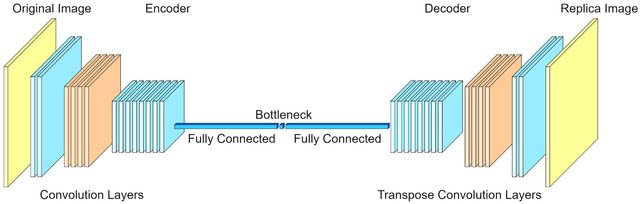
\includegraphics[width=0.9\linewidth]{./pics/bottleneck.jpg}
   \caption{Illustration of Bottleneck in Autoencoder}
\end{center}
\end{figure}

Traditionally, autoencoders are trained by requiring that the original image and the replica image are nearly the same, measured using a reconstruction loss \cite{VAEtutorial}.
After training, we can extract an encoded version of a test image by inputting the test image to the encoder and extracting the value at the bottleneck layer.

More recently, information-theoretic concepts such as mutual information and entropy have been used to better understand autoencoders \cite{infotheoretic_vaes}; and in some cases, information-theoretic concepts can even be used in place of gradient descent to train neural networks \cite{deep_infomax}.

Since information theory helps us understand and train autoencoders, we are interested in studying the information-theoretic properties of a new type of autoencoder that is built using invertible neural networks (INNs).

\section{Invertible Autoencoders}
We examine the work of Nguyen, Ardizzone, and K\"{o}the, in their paper, "Training Invertible Neural Networks as Autoencoders" \cite{Nguyen2019}.

In the following figure from Nguyen et al's work, they explain the fundamental building block of INNs: the invertible coupling layer.
Just like a ResNet is built by stacking residual blocks, INNs are built by stacking invertible coupling layers.
Theoretically, an INN can be built to any depth by stacking any number of invertible coupling layers.

\begin{figure}[!htb]
\begin{center}
   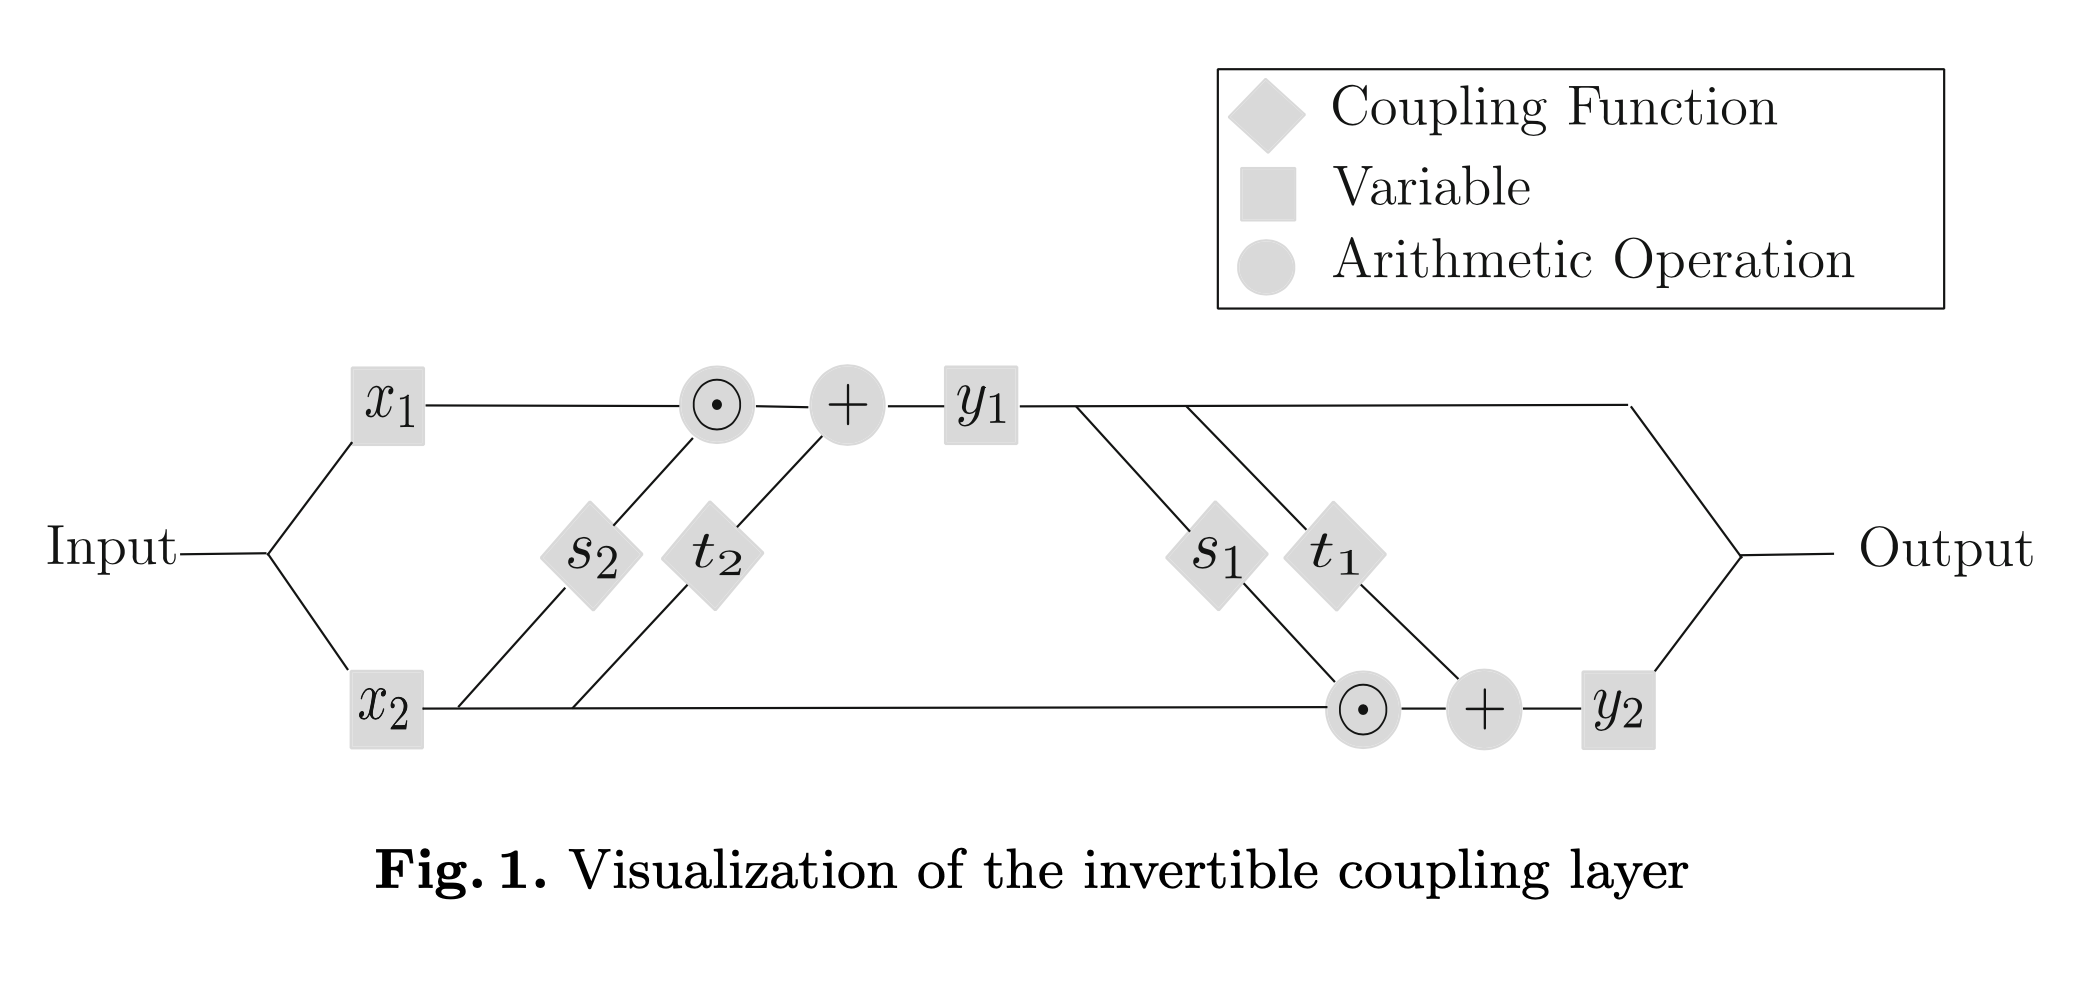
\includegraphics[width=0.9\linewidth]{./pics/invertible_coupling_layer.png}
\end{center}
\end{figure}

Although traditional neural networks are universal function approximators, INNs are limited to approximating bijective functions.
The question you might be asking, then, is this: if INNs can only approximate bijective functions, how can an INN become an autoencoder?
Since the point of an autoencoder is to encode data in a smaller-dimensional latent space, a bijection won't work, right?

The main contribution of Nguyen, et al. was to come up with a creative solution to this problem.
They do so by "zero-padding" the output of the INN.
For example, suppose our inputs have a dimension of 1000, and we wish to create a bottleneck of size 20.
To train our INN, we give it the input $ x $, obtaining $ \text{INN}(x) = y $.
Then, we replace all but the first 20 entries of $ y $ with zero, call this new output $ \hat{y} $.
Finally, we run the inverse model: $\text{INN}^{-1}(\hat{y}) = \hat{x}$.
Then, we seek to minimize the reconstruction loss \begin{align*}
    \mathscr{L}(x, \hat{x}).
\end{align*}
In so doing, we have effectively created a bottleneck.
The zero-padded $ \hat{y} $ has only 20 nonzero entries, and these entries can be thought of as our latent space encoding.

Nguyen et al. obtained very promising results.
Testing using MNIST, CIFAR-10, and CelebA, they showed that, compared to traditional autoencoders, \begin{enumerate}
   \item INNs required less training epochs;
   \item INNs could achieve smaller reconstruction losses across most bottleneck sizes;
   \item INNs required less trainable parameters than their classic autoencoder counterparts.
\end{enumerate}
The reason for 3 is primarily because the INN architecture is constant with respect to the bottleneck size, where classic autoencoders must change the number of trainable parameters depending on the bottleneck size. In their discussion of their results, they hypothesize the following
\begin{quotation}
   We already established, that if a DNN does not learn a bijective function, information loss occurs during the forward process making the inverse process ambiguous. The INN solves this ambiguity problem by introducing latent variables z containing all the information lost during the forward process.... Therefore, we hypothesize that INNs have no intrinsic information loss contrary to DNNs and the findings of Yu et al. do not apply to INNs. In other words, INNs are not bound to a maximal number of layers (depth) after which only suboptimal results can be achieved.
\end{quotation}
This is a bold hypothesis, and we will investigate it using information theory.
Primarily, we seek to answer the following questions: \begin{itemize}
   \item How much information entropy is gained or lost at each layer of the INN?
\end{itemize}


\section{Methods, Results, Discussion}

\section{Conclusion}

\pagebreak
\bibliography{references.bib}{}
\bibliographystyle{plainnat}

\end{document}
